\documentclass[10pt,a4paper]{article}
\usepackage{fontspec,polyglossia}\setmainlanguage{russian}\setmainfont{Times New Roman}
\usepackage{amsmath,amssymb,booktabs,tabularx,graphicx}\usepackage[margin=17mm]{geometry}
\usepackage[hidelinks]{hyperref}\usepackage{titlesec}\titleformat{\section}{\large\bfseries}{}{0pt}{}
\titlespacing*{\section}{0pt}{8pt}{4pt}\setlength{\parindent}{0pt}\setlength{\parskip}{4pt}\setlength{\emergencystretch}{3em}
\begin{document}
{\Large\bfseries Walker2d: единый итоговый отчёт по всей серии экспериментов с MG}\par\medskip

Восемь постановок: обучение ходьбе, стабилизация PPO, сглаживание управления, имитация и фазовое слежение. Итог на 1 октября 2026 года.

\section*{Что дала вся серия}

\textbf{Наиболее воспроизводимый результат --- MG обнаруживает упрощение выбранных управляющих логов при дообучении политики.} В двух сериях по пять парных сидов умеренное сглаживание команд сопровождается снижением MG на трёх агрегированных скалярах. Для нормы действия медианное отношение к контролю составляет 0.755 в первой серии и 0.604 во второй при одинаковом коэффициенте штрафа 1. Первая проверка управляющих логов была дополнительным анализом после опыта; в следующей серии использованы те же настройки. Это десять различных сидов дообучения, но один общий исходный навык ходьбы.

\textbf{Для полной походки получен содержательный, но пока не устойчивый по всей серии пример.} В фазовом слежении, сид 271, одновременно уменьшились ошибки повторения состояния, межцикловой разброс и усиление возмущений. MG снизился при всех пяти заданных настройках датчика и реконструкции. Совместный критерий улучшения полной походки выполнен лишь в 2/5 пар, а согласованное снижение MG при всех настройках --- в 1/5.

\textbf{Вычислительное достоинство зависит от альтернативы.} MG по сохранённому скаляру в отдельных замерах в 21--25 раз дешевле серии возмущённых симуляций, а вместе с дополнительной проверкой вложения --- в 10--11 раз. Он не заменяет их по смыслу и проигрывает по времени простым скалярным показателям. Поэтому серия поддерживает чувствительность и компактность наблюдения MG, но не универсальное превосходство метода.

\section*{Кто учится, как и что именно измеряется}

Нейросетевая политика PPO управляет шестью приводами двуногой модели Walker2d-v5 в MuJoCo. В обычной задаче она получает 17 наблюдений и учится двигаться вперёд, сохраняя допустимое положение корпуса. Стандартная награда включает скорость, бонус за здоровое состояние и штраф $0.001\|a_t\|_2^2$ за действие. В фазовых вариантах добавлены два наблюдения, sin/cos внешней фазы, и изменена задача начального запуска: удержание движения около эталонного цикла.

На выбранных этапах обучения веса фиксируются, затем агент выполняет тестовые эпизоды. MG рассчитывается по углу колена или управляющему скаляру. \textbf{Измеряется движение и управление при обученной политике, а не последовательность весов или training loss.} Различия диагностик между чекпоинтами показывают изменения поведения в ходе обучения.

Вся серия содержит 64 обучающие ветки: исходный запуск с одним продлением и 63 дообучения по 1048576 переходов. Суммарно --- 70254592 перехода по журналам основных обучений, без коротких технических тестов. Это не 64 независимых повторения одной гипотезы: сюда входят контроли, пилоты, разные вмешательства и задачи.

\section*{Общая схема сравнения}

После исходного пилота все дообучения используют отдельные сети актора/критика 64--64 с Tanh; 8 сред, rollout 512 на среду, batch 256, 5 эпох PPO, LR от $3\cdot10^{-5}$ до $3\cdot10^{-6}$, clip 0.1, target KL 0.01, $\gamma=0.99$, GAE 0.95, entropy 0, value 0.5, gradient clipping 0.5. Нормировки заморожены, лимит обучающего эпизода 5000 шагов. Общая исходная политика --- ранний устойчивый checkpoint исходного сида 200 после 655360 переходов. Для фазовых входов добавлены нулевые веса и одинаково сброшен Adam.

Тестовая запись: детерминированная политика, 512 шагов разогрева и 4096 анализа, шаг управления 0.008 с. Требуются отсутствие падения и скорость не ниже 0.5; для сравнения логов --- также std правого колена не ниже 0.05 и минимум восемь пиков (prominence 0.15, расстояние 20). Награда делится на фиксированные 4096 шагов с нулевым остатком после падения. MG не получает нулевую оценку вместо неудачного эпизода: такие записи исключаются из парного анализа и остаются в статистике качества.

Основной MG: окно 2048, задержка 8, вложение 20, 20 соседей, Theiler 312; проверка вложения 40. В ранней repair-серии пять окон с шагом 512, в последующих обычно три окна с концами 2048,3072,4096. Для проверки датчика и масштаба сохранены альтернативные окна, задержки и левое колено. Настройки, определения и наборы reset различаются между ветками; ниже сравнения всегда делаются внутри соответствующей постановки.

\newpage

\section*{Все восемь постановок: что пробовали и что получили}

Число обучений включает пилоты и контроли. Подтверждающий повтор --- отдельный сид дообучения; десять тестовых reset одной политики не являются десятью обучениями.

\begin{center}\small
\begin{tabularx}{\linewidth}{l>{\raggedright\arraybackslash}X>{\raggedright\arraybackslash}X}
\toprule
Ветка / обучения & Проверяемое изменение & Итог \\
\midrule
Исходная ходьба / 1 & PPO с нуля, без навязывания регулярности & После 4194304 переходов пригодны 0/3 финальных записей. MG и подтверждающая серия не запускались. \\
Стабилизация / 6 & Более осторожное дообучение ранней ходящей политики & Критерий стабильности прошли 4/5 сидов, финальная ходьба 47/50. Совместного улучшения полной походки --- 0/5; основной MG не снижался. \\
Сглаживание / 12 & Штраф на изменение средней команды, коэффициент 0/1 & J1/J2 уменьшились; коленный MG снизился описательно в 5/5, но полного улучшения с сохранением качества --- 0/5. Дополнительный анализ управляющих логов дал устойчивый положительный результат. \\
Имитация / 3 & Приближение к циклу без внешних часов, коэффициенты 0/1/3 & На одном пилотном сиде ни один штраф не прошёл отбор. При коэффициенте 1 R/D ухудшились до 2.09/6.32 от контроля. \\
Фазовое слежение / 2 & Ошибка до точки цикла с известной фазой, коэффициент 0/3 & Узкий штраф почти насыщался. На тесте R=0.746, D=1.015, MG=1.053: согласованного улучшения нет. \\
Расширенный штраф слежения / 12 & Исправлен масштаб ошибки, затем пять новых пар & Критерий полного улучшения --- 2/5; основной MG ниже в 3/5. Сид 271 согласован по всем пяти настройкам MG и независимым метрикам. \\
Слежение + сглаживание / 4 & Пилот 2\ensuremath{\times}2: слежение 0/3 и сглаживание 0/1 & Все варианты ходят в 5/5 validation-эпизодах, но совместный критерий R и разброса по циклу не пройден. Расширения на пять сидов нет. \\
Сила сглаживания / 24 & Четыре коэффициента 0/0.25/1/4, пилот и пять новых сидов & Умеренные штрафы снижают MG агрегированных логов на 5/5 сидов. Сильный штраф ухудшает ходьбу; MG нормы действия обычно растёт. \\
\bottomrule\end{tabularx}\end{center}

В первой строке 0/3 относится к числу пригодных финальных записей, а не к проверке MG. Неудача формирования нужной пары движений не считается неудачей оценщика.

\section*{Два разных способа вмешательства}

\textbf{Сглаживание управления} добавляет к PPO-loss средний квадрат разности ограниченных средних действий на соседних состояниях:

\[
L=L_{\rm PPO}+\frac{\lambda}{6}\,\mathbb E\|\bar a_\theta(s_{t+1})-\bar a_\theta(s_t)\|_2^2,
\qquad \bar a_\theta=\operatorname{clip}(\mu_\theta,-1,1).
\]

Границы эпизодов исключены из пар, исследовательский шум не штрафуется, награда среды прежняя. При исполнении нет дополнительного фильтра команд. Здесь ожидается прежде всего упрощение управления; повторяемость полного тела проверяется отдельно.

\textbf{Имитация и слежение} изменяют награду: $r'_t=r_t-\lambda(1-\exp[-e_t^2/(2\sigma^2)])$. Эталон --- наблюдавшийся цикл исходной политики длиной 152 шага. Без фазы $e_t$ --- расстояние до ближайшей точки цикла; с фазой --- до заданной точки. В фазовых опытах агент стартует около случайной точки цикла, получает sin/cos часов, а период внешнего сигнала составляет около 152.215 шага. Это локальное удержание походки с внешним воздействием, а не обычный старт Walker2d из вертикального положения.

Исходный масштаб $\sigma^2=0.116779$ давал насыщение штрафа. В следующем пилоте его заменили на 38.477 по validation-ошибкам контроля, до просмотра MG. Пилот прошёл отбор, поэтому были выполнены все пять пар 271--275. Подстройка масштаба и разные варианты одного пилота не считаются независимыми подтверждениями.

В совместном пилоте 280 добавление сглаживания к слежению уменьшило J1 примерно до трети, но разброс по всему циклу не улучшился: медианы C составили 0.932 у слежения и 0.948 у сочетания. Это сохранённый отрицательный контроль против отождествления гладких команд и простой физической траектории.

\newpage

\section*{Главный воспроизводимый результат: упрощение управляющих логов}

В первой парной серии 221--225 после исходного анализа коленного датчика были проверены логи действий. Норма команды, норма её приращения и среднее шести команд дали одинаковый знак на всех пяти сидах. В следующей серии 231--235 эта постановка воспроизведена с теми же настройками MG. В таблице --- медианы отношений сглаживания к контролю при коэффициенте 1.

\begin{center}\small
\begin{tabularx}{\linewidth}{l>{\raggedright\arraybackslash}X>{\raggedright\arraybackslash}X}
\toprule
Скалярный лог & Первая серия: отношение / снижение & Следующая серия: отношение / снижение \\
\midrule
Норма команды & \textbf{0.755 / 5 из 5} & \textbf{0.604 / 5 из 5} \\
Норма приращения & \textbf{0.717 / 5 из 5} & \textbf{0.601 / 5 из 5} \\
Среднее шести команд & \textbf{0.758 / 5 из 5} & \textbf{0.651 / 5 из 5} \\
\bottomrule\end{tabularx}\end{center}

\begin{center}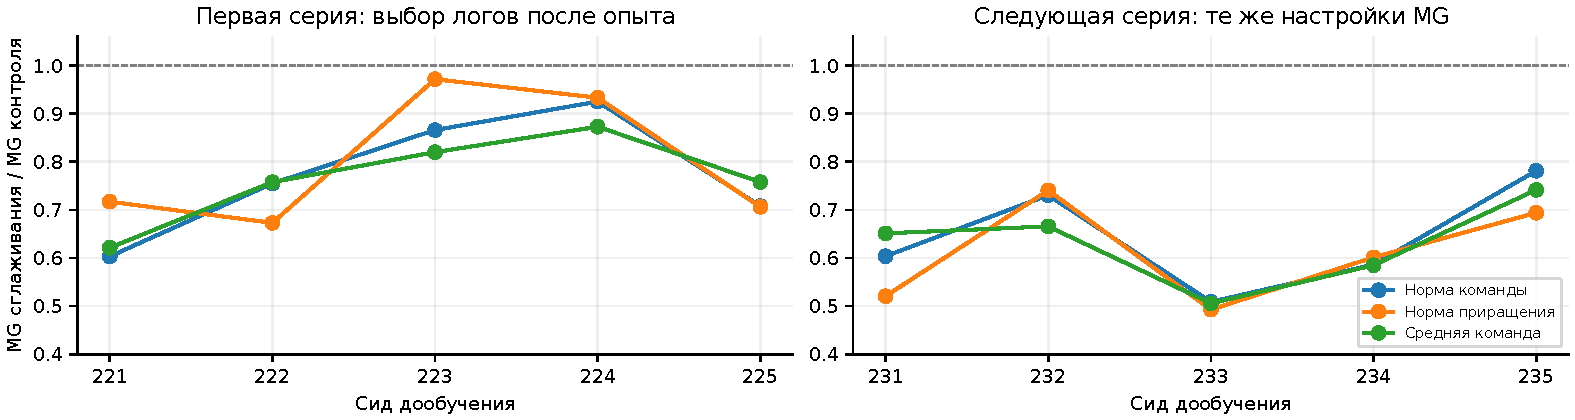
\includegraphics[width=\linewidth,height=.32\textheight,keepaspectratio]{control_logs.pdf}\end{center}

Это наиболее сильное свидетельство воспроизводимости скалярного сигнала в Walker2d: знак сохраняется для трёх агрегатов на каждом сиде. Логи коррелированы, исходная политика общая, первая проверка была после просмотра результатов. У сида222 лишь шесть общих записей вместо исходно требовавшихся восьми: его сравнение описательное. Таблица не даёт 30 независимых подтверждений.

\textbf{Независимый смысл изменения.} $J_1$ и $J_2$ --- средние по времени и шести каналам квадраты первой и второй разности команд. При умеренном штрафе оба падают. Это подтверждает более плавное управление, хотя J1 близок к обучающему штрафу. В первой серии медиана J1 около 0.35 от контроля; во второй при коэффициенте 1 ---0.331. Изменение управления видно без MG, а MG воспроизводимо отражает его по одному скаляру.

\section*{Граница полезного сглаживания}

Пять новых сидов проверены при четырёх коэффициентах. MG относится к норме команды; награда учитывает все 50 эпизодов, включая падения, и дана как отношение средних. MG/J1/J2 --- медианы парных отношений внутри сида, затем по пяти сидам.

\begin{center}\small
\begin{tabularx}{\linewidth}{l>{\raggedright\arraybackslash}X>{\raggedright\arraybackslash}X>{\raggedright\arraybackslash}X>{\raggedright\arraybackslash}X>{\raggedright\arraybackslash}X}
\toprule
Штраф & Ходьба & Награда & MG & J1 & J2 \\
\midrule
0 & 48/50 & 1.000 & 1.000 & 1.000 & 1.000 \\
0.25 & 49/50 & 1.020 & 0.801 & 0.539 & 0.385 \\
1 & 47/50 & 0.978 & 0.604 & 0.331 & 0.181 \\
4 & 25/50 & 0.681 & 1.114 & 0.180 & 0.064 \\
\bottomrule\end{tabularx}\end{center}

При коэффициенте 4 команды ещё плавнее, но качество ухудшается и MG нормы команды растёт относительно контроля на 4/5 сидов. На одинаковых пригодных reset коэффициентов 0,1,4 отношение MG сильного штрафа к умеренному равно 1.704, рост на 5/5 сидов. Значит, MG не просто повторяет величину соседних приращений. Этот контраст не является обученным детектором отказов; анализ относится к сохранившим ходьбу эпизодам.

Промежуточные чекпоинты также показывают изменение. Для коэффициента 0.25 на фиксированном reset 62001 отношение MG составило 1.000,0.811,0.808,0.747,0.745 после 0,262144,524288,786432,1048576 переходов. Пригодных пар соответственно 5,5,5,4,5. MG может использоваться для периодической проверки поведения по мере обучения; монотонность и раннее предсказание качества не установлены.

При этом \textbf{снижение MG управляющего или коленного лога не означает автоматического улучшения всего движения}. В первой серии, сид 223, J1=0.209 и коленный MG=0.696 от контроля, но ошибка повторения тела выросла в 2.23 раза, фазовый разброс ---в 2.81. Обе политики прошли все десять эпизодов. Это реальное расхождение свойств, а не результат исключения падений.

\newpage

\section*{Что подтверждено для полной походки}

Независимые диагностики используют 17 физических координат: восемь положений без абсолютного горизонтального продвижения и девять скоростей, делённых на 5. Пусть $V$ --- средний квадрат расстояния состояния от его среднего. R --- минимум среднего квадрата $x_{t+p}-x_t$ по лагам 20--250, делённого на $2V$. D --- дисперсия состояния в выбранном сечении, делённая на V. В ранних опытах сечение задавали пики колена; в имитации --- фиксированная плоскость; в фазовом слежении --- внешняя фаза 0. Абсолютные D между этими задачами несопоставимы.

C --- разброс состояний между циклами после интерполяции на 64 одинаковые фазы, усреднённый по всему циклу и нормированный на V. Его добавили после первых результатов фазовой серии; он не заменяет заранее заданный критерий. Сильное событие в подтверждении слежения требует обоих отношений R,D не выше 0.75, минимум восьми общих записей и сохранения качества. В ранней repair-серии критерий отличается деталями; полные условия сохранены в протоколах.

Все числа в следующей таблице --- отношения слежения к собственному контролю; меньше единицы означает снижение показателя.

\begin{center}\small
\begin{tabularx}{\linewidth}{l>{\raggedright\arraybackslash}X>{\raggedright\arraybackslash}X>{\raggedright\arraybackslash}X>{\raggedright\arraybackslash}X>{\raggedright\arraybackslash}X}
\toprule
Сид слежения & R & D & C & MG правого колена & Совместный критерий \\
\midrule
271 & 0.532 & 0.074 & 0.624 & 0.872 & \textbf{Да} \\
272 & 0.546 & 1.055 & 1.003 & 1.159 & Нет \\
273 & 0.297 & 1.189 & 0.998 & 0.913 & Нет \\
274 & 1.119 & 0.104 & 0.753 & 1.087 & Нет \\
275 & 0.682 & 0.482 & 0.829 & 0.975 & \textbf{Да} \\
\bottomrule\end{tabularx}\end{center}

\begin{center}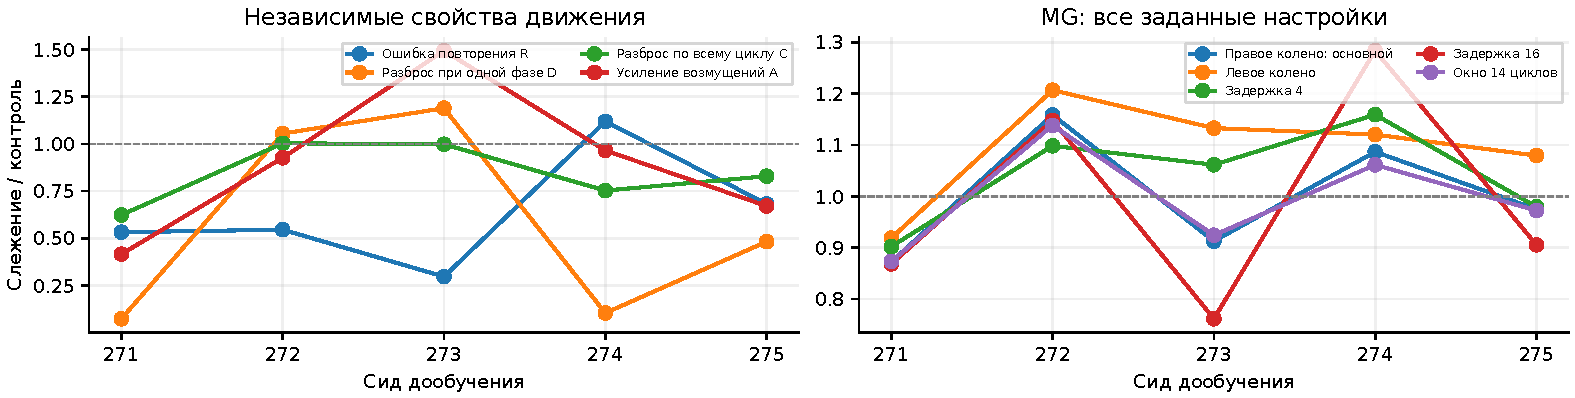
\includegraphics[width=\linewidth,height=.32\textheight,keepaspectratio]{whole_gait.pdf}\end{center}

\textbf{Сид 271 --- сильный согласованный пример.} Награда сохранена (отношение 1.005), ходьба 10/10 у обеих политик. R снизился на 47\%, D на 93\%, C на 38\%. Основной MG снизился на 13\%; при левом колене, задержках 4/16 и окне 14 циклов снижение составляет 8--13\%. Усиление возмущений на одной проверенной траектории снизилось до 0.416 от контроля. Таким образом, скалярный MG согласуется с несколькими независимо вычисляемыми характеристиками полной системы.

Этот пример выбран для иллюстрации после анализа всей серии. В сиде 275 R/D также улучшились, но MG левого колена вырос. Во всей серии основной MG уменьшился в 3/5 пар, во всех пяти настройках --- в 1/5. Дополнительные среднее и разность углов колен также не дали общего снижения на всех сидах. Спектральная энтропия в сиде 271 тоже снизилась, поэтому уникальность диагностической способности MG здесь не показана.

\section*{Что измеряли дорогими пробами и почему это не спектр Ляпунова}

Для каждой пары на одном заранее выбранном общем reset выполняли 68 возмущённых продолжений:17 координат, два знака, две точки траектории, величина 0.001 в масштабированных координатах. В окончательной сопоставимой проверке горизонт 600 шагов, или 4.8с; политика заново выбирает действия. A --- медианное конечновременное усиление расстояния. В автономных задачах разрешено выравнивание фазы, в задачах с внешними часами сравниваются одинаковые фазы. Для сида 274 слежение дало 3 падения из 68 проб; их не скрывали за медианой A.

Конечными разностями также оценивались матрицы локального отображения через 152 шага. При уменьшении шага возмущения матрицы менялись примерно на свою норму (относительные различия около 1.00 и 1.08 на первой паре). Кроме того, заданный период около 152.215 не равен 152 и периодическая орбита не доказана. Поэтому эти спектры не использованы как надёжная истина о размерности или устойчивости. Сравнение с пробами A --- сравнение разных диагностик, не доказательство замены спектра MG.

\newpage

\section*{Вычислительные преимущества и сравнение с дешёвыми методами}

Время ниже измерено отдельными последовательными CPU-запусками после обучения, по одному численному потоку. MG и дешёвые методы обрабатывают одинаковые три окна 2048; возмущения требуют дополнительных симуляций. Загрузка модели исключена. Между сериями замеры не являются единым аппаратным тестом; корректно сравнивать методы внутри столбца.

\begin{center}\small
\begin{tabularx}{\linewidth}{l>{\raggedright\arraybackslash}X>{\raggedright\arraybackslash}X}
\toprule
Расчёт & Сглаживание, с & Фазовое слежение, с \\
\midrule
MG, вложение 20 & 1.010 & 0.636 \\
MG с проверкой вложения 40 & 2.207 & 1.330 \\
Полносостоянийные показатели & 0.065 & 0.043 \\
Простые скалярные признаки & 0.013 & 0.004 \\
68 возмущений; в фазовой серии также матрицы & 24.945 & 13.670 \\
Получение общей исходной записи, отдельно & 2.767 & 1.405 \\
\bottomrule\end{tabularx}\end{center}

\textbf{MG без дополнительной проверки дешевле дорогих проб примерно в 24.7 и 21.5 раза; с проверкой --- в 11.3 и 10.3 раза.} Это его измеренное вычислительное достоинство в данной серии: анализ уже имеющегося скаляра требует существенно меньше вычислений, чем многократные вмешательства в симуляцию. Возможность выбирать с помощью MG моменты для дорогой диагностики остаётся гипотезой: такой алгоритм отбора здесь не проверялся.

Сравнение с простыми показателями обязательно. Финальная проверка использовала тот же скаляр нормы команды и те же окна. H --- нормированная спектральная энтропия; Q --- средний квадрат соседнего приращения / удвоенная дисперсия; $R_x$ --- аналогично нормированная ошибка возврата скаляра с лучшим лагом 20--250. В таблице: отношение к контролю и число сидов со снижением.

\begin{center}\small
\begin{tabularx}{\linewidth}{l>{\raggedright\arraybackslash}X>{\raggedright\arraybackslash}X>{\raggedright\arraybackslash}X}
\toprule
Метод & Слабый штраф 0.25 & Умеренный штраф 1 & Время одного окна \\
\midrule
\textbf{MG} & \textbf{0.801; 5/5} & \textbf{0.604; 5/5} & 369 мс \\
Энтропия H & 0.996; 4/5 & 0.958; 3/5 & 0.103 мс \\
Повторение $R_x$ & 0.799; 4/5 & 0.790; 5/5 & 3.782 мс \\
Приращения Q & 0.809; 4/5 & 0.598; 5/5 & 0.048 мс \\
\bottomrule\end{tabularx}\end{center}

MG показывает более устойчивый знак при слабом вмешательстве основного лога, особенно по сравнению с энтропией. Преимущество 5/5 против 4/5 при пяти сидах описательное, не установленное статистическое превосходство. $R_x$ тоже обнаруживает нарушение повторяемости при сильном штрафе, а на дополнительных логах хорошо реагирует и на умеренный штраф. В этой реализации он примерно в 98 раз быстрее MG. Все четыре метода используют один скаляр: компактность наблюдения не является исключительным достоинством MG перед этими конкурентами.

\section*{Проверки, определяющие корректную интерпретацию всей серии}

\textbf{Временной масштаб важен.} После стабилизации PPO основной коленный MG вырос во всех пяти сидах. Анализ с окнами, согласованными по числу циклов, и ресэмплингом менял знак в части повторов. Период для этой диагностики получали из полного состояния: это дополнительная информация, не автономный скалярный алгоритм. Ранние пробы длиной 4P также имели разный физический горизонт; для последующих выводов использованы исправленные пробы по 600 шагов. Старые значения сохранены, а более удобные настройки не подменяют основные.

\textbf{Проверено качество вычислений:} общие начальные и разные конечные веса, неизменные нормировки, точное невозмущённое воспроизведение, совпадение нулевого штрафа с PPO на коротком тесте, пересчёт метрик из сырых данных. Неудачные пилоты и исключённые эпизоды сохранены. Чувствительность к окну и вложению не позволяет считать абсолютный MG истинным числом компонент.

\section*{Общий вывод для статьи}

\textbf{Серия Walker2d показывает, что MG применим как скалярный индикатор изменения временной структуры поведения обучаемой политики. Самый устойчивый результат --- снижение оценки на агрегированных управляющих логах при умеренном сглаживании, воспроизведённое в двух сериях по пять сидов. Получен также отдельный согласованный пример упрощения полной походки с независимыми проверками состояния и возмущений. MG существенно дешевле многократных возмущённых симуляций, но не заменяет их и уступает простым скалярным показателям по времени.}

Упрощение команд, повторяемость тела, награда и устойчивость к возмущениям --- разные свойства. Общая исходная политика ограничивает переносимость. MG здесь --- дополнительный анализатор конкретного лога; универсальность, точное определение размерности и прогнозирование отказов не установлены. Источники всех восьми веток и команды сборки: README.md. Статья не изменялась.
\end{document}